\section{Раработка программного обеспечения}

\subsection{Разработка серверной части}

Структура приложения, написанного на фреймворке Django представляет собой набор отдельных приложений, выполняющих отдельные функции.
Каждое приложение вклбчает в себя:
\begin{itemize}
    \item models.py - файл, содержащий представление моделей базы данных;
    \item migrations/ - папка, хранящая миграции моделей;
    \item serialzers.py - файл, содержащий представления входных/выходных данных сервера;
    \item views.py - файл, содержащий контроллеры, обрабатывающие запросы;
    \item utils.py - файл, содержащий вспомогательные функции приложения, например сервисы обращения к третьим приложения;
    \item tasks.py - файл, содержищий асинхронные-задачи данного приложения, которые взаимодействуют с моделями это приложения, либо логически относятся к нему;
    \item tests.py - файл, содержащий тесты к контроллерам;
    \item factories.py - файл, содержащий фабрики для генерации данных для тестов;
    \item permissions.py - файл, содержащий пользовательские разрешения для запросов;
    \item signals.py - файл, содержащий сигналы для моделей БД;
    \item admin.py - файл, содержаший модели представления и модификации сайта администратора;
    \item urls.py - файл, содержищий связи между контроллерами и url-адресами.
\end{itemize}

Хоть Django фреймворк и предоставляет готовую структуру для написания веб-приложения, однако в каждом проекте присутствуют утилиты, нужные в независимости от приложения.
К таким утилитам относятся работы со структурами данных, работа с изображениями и интернализацией, миксины для контроллеров, сериализаторов либо тестов и тд.
Для таких утилит на уровне приложений была создана отдельная папка <<utils>>, содержащая модули python, разбитые по категориям:
\begin{itemize}
    \item strings.py - файл, содержащий утилиты для работы со строками;
    \item tests.py - папка, содержащий утилиты для работы с тестами;
    \item constants.py - файл, содержащий константы приложения;
    \item mixins.py - файл, содержащий миксины для сериализаторов и контроллеров;
    \item images.py - файл, содержащий утилиты для работы с изображениями;
    \item i18l.py - файл, содержащий утилиты для рабоыт с интернализацией;
    \item models.py - файл, содержащий утилиты для рабоыт с моделями.
\end{itemize}

Для предоставления возможности масштабирования системы была выбрана плоская структура конечных точек HTTP[19].
Данная структура характеризуется большим объемом мелких конечных точек, отвечающих за отдельные сущность.
Одновременно минусом и плюсом данной структуры является, как оговаривалось раньше, возможность получения конкретных объектов базы данных по средством отдельных конечных точек.
Таким образом, например, для получения всех данных о пользователе, клиент должен будеть послать несколько запросов к серверу.
Данная архитектура увеличивает количество запросов к серверу, однако сложно представить, что на одной странице клиента будут отображены все данные о пользователе.
И при нескольких конечных точках возможно, при ее необходимости, закгрузка данных в фоне.

На основании выбора плоской архитектуры к организации программного интерфейса к серверной части приложения были реализованы приложения: Auth, Users, Goods, Payments, Orders, Addresses (таблица 4.1).
Итоговая структура проекта представлена на рисунке \ref{back:struct}.

\begin{figure}[h!]
    \begin{subfigure}[b]{0.3\textwidth}
    \centering
    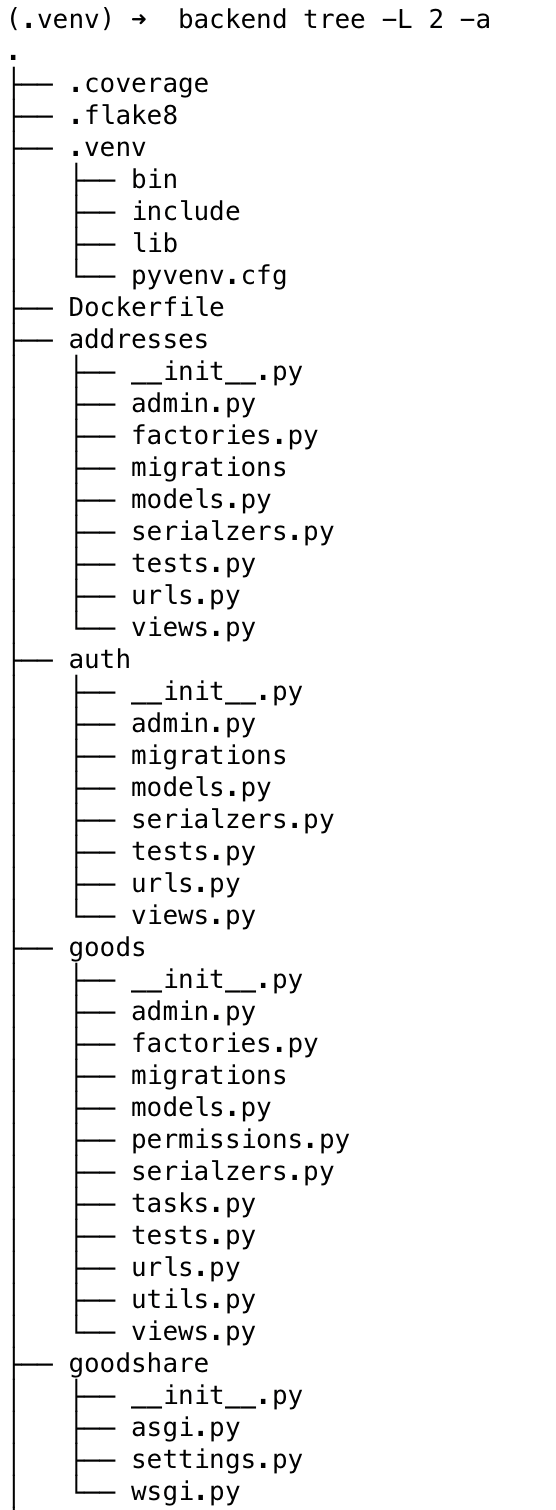
\includegraphics[scale=0.8]{structure_1.png}
    \caption{}
    \end{subfigure}
    \begin{subfigure}[b]{0.3\textwidth}
    \centering
    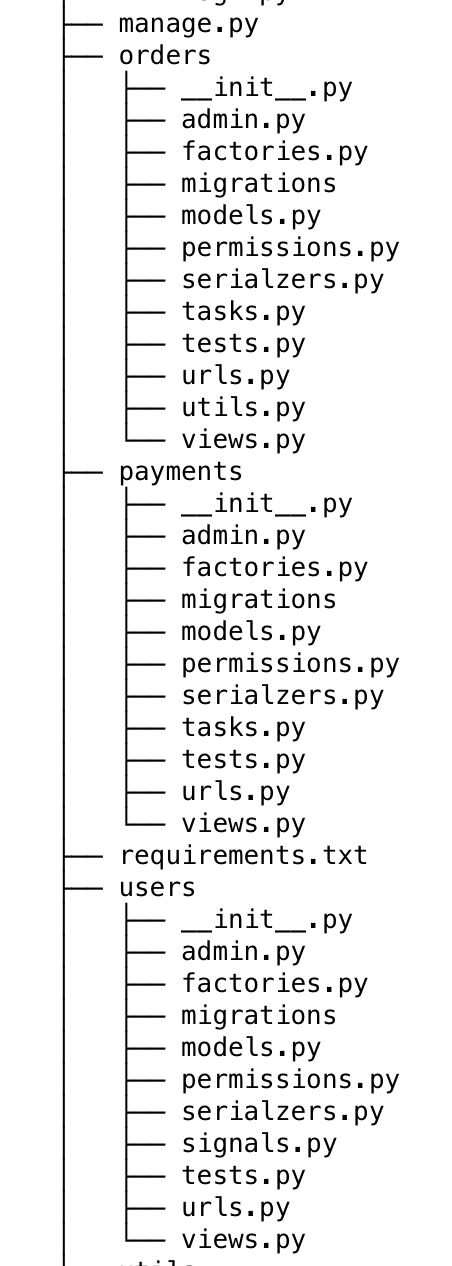
\includegraphics[scale=0.8]{structure_2.png}
    \caption{}
    \end{subfigure}
    \begin{subfigure}[b]{0.3\textwidth}
    \centering
    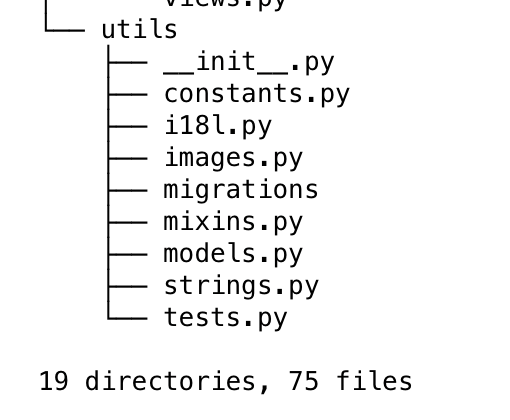
\includegraphics[scale=0.8]{structure_3.png}
    \caption{}
    \end{subfigure}
    \caption{ Структура серверной части приложения }
    \label{back:struct}
\end{figure}

\begin{table}
    \caption{Приложения серверной части}
    \begin{tabular}{ | l | p{6cm} | }
        \hline
        Название приложения & Выполняющие функции \\ \hline
        Auth & Отвечает за процесс авторизации пользователя в системе \\ \hline
        Users & Отвечает за манипуляции с пользовательскими данными \\ \hline
        Goods & Отвечает за доступ к товарам и взаимодействия с ними \\ \hline
        Payments & Хранения сохранненых данных для оплаты пользователя\\ \hline
        Orders & Хранения и соверщение заказов пользователя \\ \hline
        Addresses & Хранения адресов оплаты пользователя \\ \hline
    \end{tabular}
\end{table}


\subsubsection{Программный интерфейс серверной части}\hfill

На основании функциональных требований в каждом приложении были реализованы API конечных точек HTTP-запросов (таблицы 4.2-4.7).

\begin{table}
    \caption{Приложение Auth, базовый url адрес конечных точек <</auth>>}
    \begin{tabular}{ | p{3cm} | p{4cm} | p{3cm} | p{3cm} | }
        \hline
        url-адрес запроса / метод запроса & входные данные & выходные данные  & описание \\ \hline
    /verify POST  & phone - номер телефона, token - токен, выданные firebase, после вводна OTP кода & token - токен авторизации пользователя для осузествления запросов к серверу & С помощью данного запроса пользователь может авторизироваться в приложении с помощью токена \\ \hline
    \end{tabular}
\end{table}

\begin{table}
    \caption{Приложение Users, базовый url адрес конечных точек <</users>>}
    \begin{tabular}{ | p{3cm} | p{4cm} | p{3cm} | p{3cm} | }
        \hline
        url-адрес запроса / метод запроса & входные данные & выходные данные  & описание \\ \hline
        / POST & name - ФИО пользователя, photo - фото пользователя & созданная модель пользователя & создание пользователя в системе \\ \hline
        / PUT & name - ФИО пользователя, photo - фото пользователя, email - электронная почта пользователя & обновленная модель пользователя & обновление данных пользователя \\ \hline
        /ID/review POST & text - текст отзыва, mark - оценка пользователя & & создание отзыва о пользователе \\ \hline
        / GET & & получение информации о пользователе \\ \hline
    \end{tabular}
\end{table}

\begin{table}
    \caption{Приложение Addresses, базовый url адрес конечных точек <</addresses>>}
    \begin{tabular}{ | p{3cm} | p{4cm} | p{3cm} | p{3cm} | }
        \hline
        url-адрес запроса / метод запроса & входные данные & выходные данные  & описание \\ \hline
        / POST & city - город получателя, street - улица получателя, building - номер здания получателя, appartament - номер квартиры получателя & созданная модель адреса & создания адреса доставки пользователя \\ \hline
        /ID PUT & city - город получателя, street - улица получателя, building - номер здания получателя, appartament - номер квартиры получателя & обновленная модель адреса & обновление адреса доставки пользователя \\ \hline
        /ID DELETE & & & удаление адреса доставки пользователя \\ \hline
        / GET & & & получение всех сохраенных записей адресов \\ \hline
    \end{tabular}
\end{table}

\begin{table}
    \caption{Приложение Payments, базовый url адрес конечных точек <</payments>>}
    \begin{tabular}{ | p{3cm} | p{4cm} | p{3cm} | p{3cm} | }
        \hline
        url-адрес запроса / метод запроса & входные данные & выходные данные  & описание \\ \hline
        / POST & card\_number - номер карты пользователя, cvv\_code - cvv-код карты, date\_expire - срок годности карты, cardholder\_name - имя держателя карты & созданная модель оплаты & создание модели оплаты пользователя \\ \hline
        /ID PUT & card\_number - номер карты пользователя, cvv\_code - cvv-код карты, date\_expire - срок годности карты, cardholder\_name - имя держателя карты & обновленная модель оплаты & обновление модели оплаты пользователя \\ \hline
        /ID DELETE & & & удаление модели оплаты \\ \hline
        / GET & & & получение всех сохраенных записей оплат \\ \hline
    \end{tabular}
\end{table}

\begin{table}
    \caption{Приложение Goods, базовый url адрес конечных точек <</goods>>}
    \begin{tabular}{ | p{3cm} | p{4cm} | p{3cm} | p{3cm} | }
        \hline
        url-адрес запроса / метод запроса & входные данные & выходные данные  & описание \\ \hline
        /add POST & name - название товара, condition - состояние товара, description - описание товара, can\_be\_purchased - возможность выкупа товара, price\_per\_hour - цена аренды товара за час, price\_per\_day - цена аренды товара за сутки, own\_deliver - возможность доставки товара арендадателем & созданная модель товара & создания товара \\ \hline
        /ID PUT & name - название товара, condition - состояние товара, description - описание товара, can\_be\_purchased - возможность выкупа товара, price\_per\_hour - цена аренды товара за час, price\_per\_day - цена аренды товара за сутки, own\_deliver - возможность доставки товара арендадателем & обновленная модель товара & обновление информации о товаре \\ \hline
        /ID DELETE & & & удаление товара \\ \hline
        /ID/add-to-basket PUT &  & & добавление товара в корзину \\ \hline
        /ID/remove-from-basket PUT & & & удаление товара из корзины \\ \hline
        /?page=PAGE GET & PAGE - страница поисков & список моделей товаров & получить все товары \\ \hline
        /?page=PAGE \&XX=YY GET & PAGE - страница поисков, XX=элемент фильтрации, YY -  значение XX фильтра & список моделей товаров & получить все товары \\ \hline
    \end{tabular}
\end{table}

\begin{table}
    \caption{Приложение Orders, базовый url адрес конечных точек <</orders>>}
    \begin{tabular}{ | p{3cm} | p{4cm} | p{3cm} | p{3cm} | }
        \hline
        / POST & start\_use\_date - дата начала пользования, end\_use\_date - дата окончания пользования, payment - выбор оплаты, address - выбор адреса доставки & модель заказа & создание заказа \\ \hline
        /ID/pay PUT & & & оплата товара; \\ \hline
        / GET & & список моделей заказов & получение списка заказов. \\ \hline
    \end{tabular}
\end{table}

\subsection{Разработка клиентской части}

Как было описано в разделе про проектирование клиентской части, в среде React приложений нет четко выработанной структуры приложений.
Однако основываясь на практиках написания React приложений была реализованна структура приложения, представленная на рисунке \ref{front:struct}.

Глобальное состояние приложения была разделено на несколько редьюсеров:
\begin{itemize}
    \item appReducer - котнролирует глобальное состояние приложение, а именно контроль отображения загрузчиков в приложении;
    \item authReducer - контролирует изменение и процесс аунтентификации пользователя;
    \item basketReducer - контролирует состояние корзины пользователя;
    \item checkoutReducer - контролирует процесс покупки товара;
    \item filterReducer - отвечает за фильтрацию товаров на экране поиска товаров;
    \item productReducer - отвечает за создание и изменения пользовательских продуктов;
    \item profileReducer - отвечает за состяние пользовательских данных;
    \item orderReducer - отвечает за состояние пользовательских заказов;
\end{itemize}

Соответственно каждому редьюсеру были созданы саги, экшены и константы, которые провоцируют приложению на осуществление запросов на сервер либо изменение состояния.

Компоненты приложения расположены в директориях <<components>> и <<views>> таким образом, что в директории <<components>> расположены глупые компоненты, представляющие репрезентационные компоненты.
А в дирректории <<views>> расположены как экраны приложения, так и компоненты-контейнеры.
\begin{figure}[h]
    \begin{subfigure}[b]{0.45\textwidth}
    \centering
    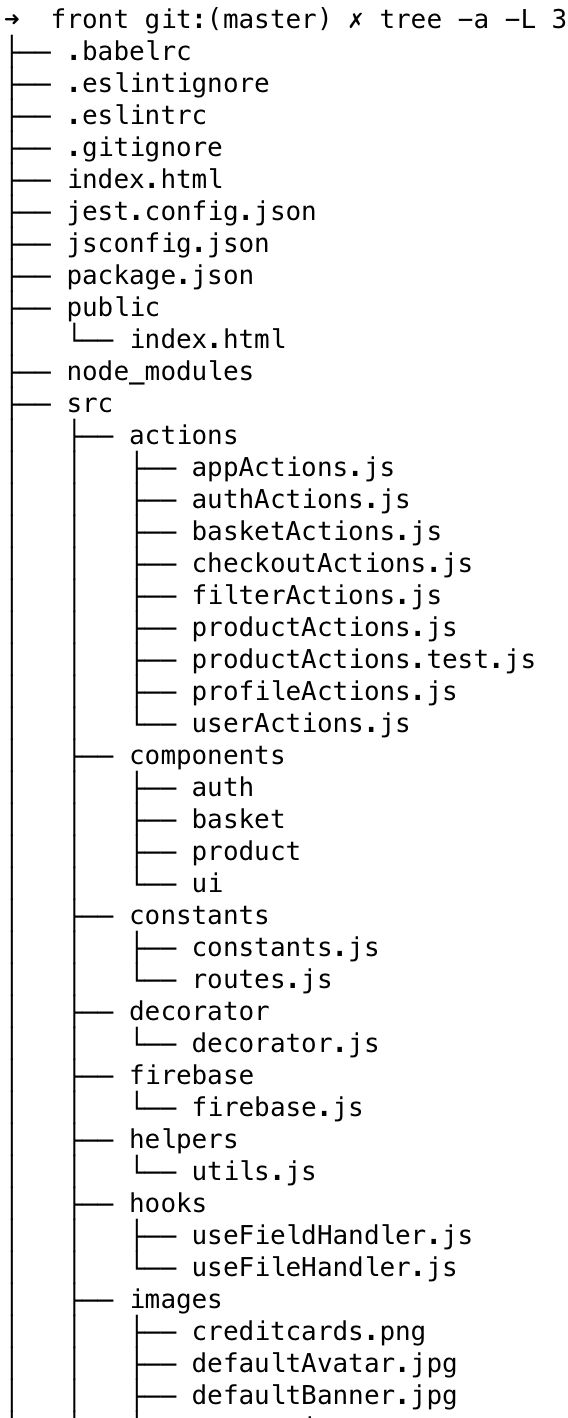
\includegraphics[scale=0.8]{front_structure_1.png}
    \caption{}
    \end{subfigure}
    \begin{subfigure}[b]{0.3\textwidth}
    \centering
    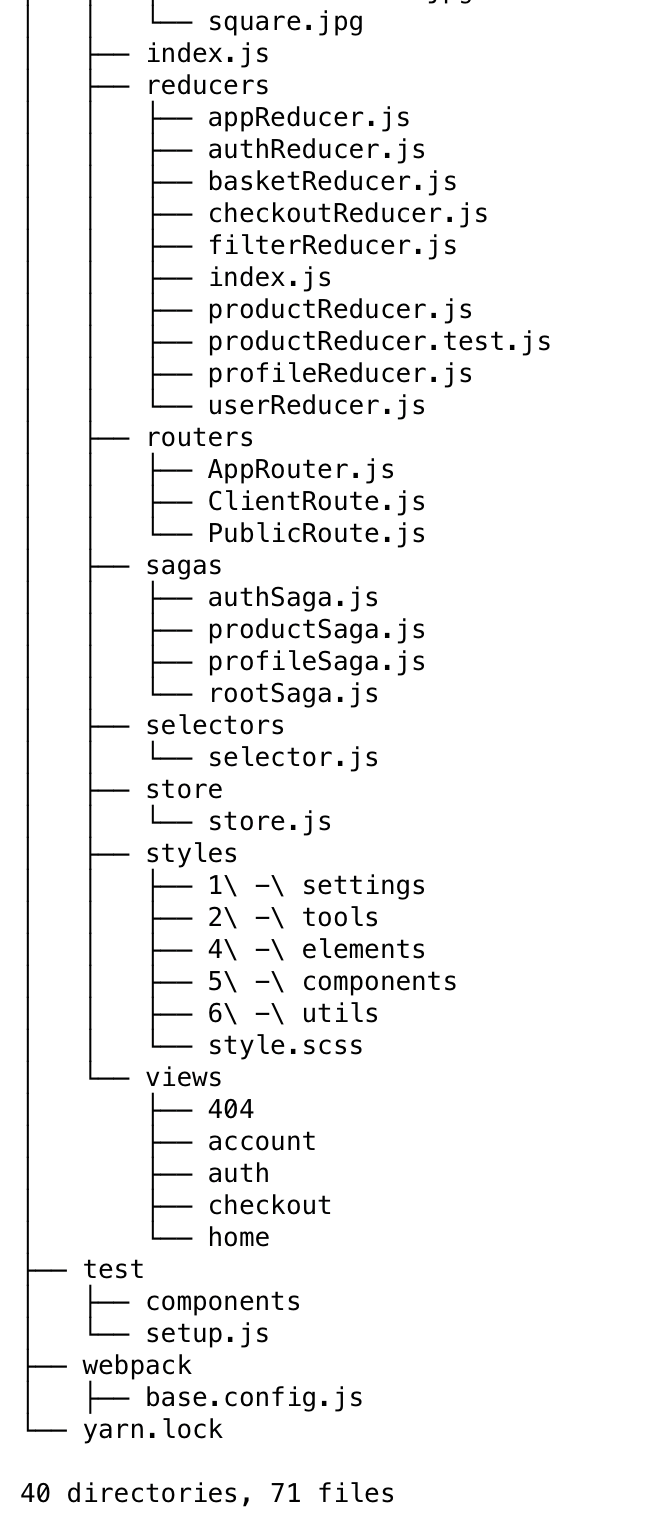
\includegraphics[scale=0.8]{front_structure_2.png}
    \caption{}
    \end{subfigure}
    \caption{ Структура клиентской части приложения }
    \label{front:struct}
\end{figure}

В главе про проектирование было


\subsection{Интеграция Firebase}
В данном проекте из платформы Firebase использовались 2 модуля:
\begin{itemize}
    \item Authentication;
    \item Messaging.
\end{itemize}

На серверной части интеграция с Firebase происходит с помощью пакета firebase-admin.
Для инициализации Firebase проекта на серверной части необходимо скачать сервисный файл с панели администратора на Firebase(см рисунок \ref{fire:admin}).

\begin{figure}[ht]
    \centering
    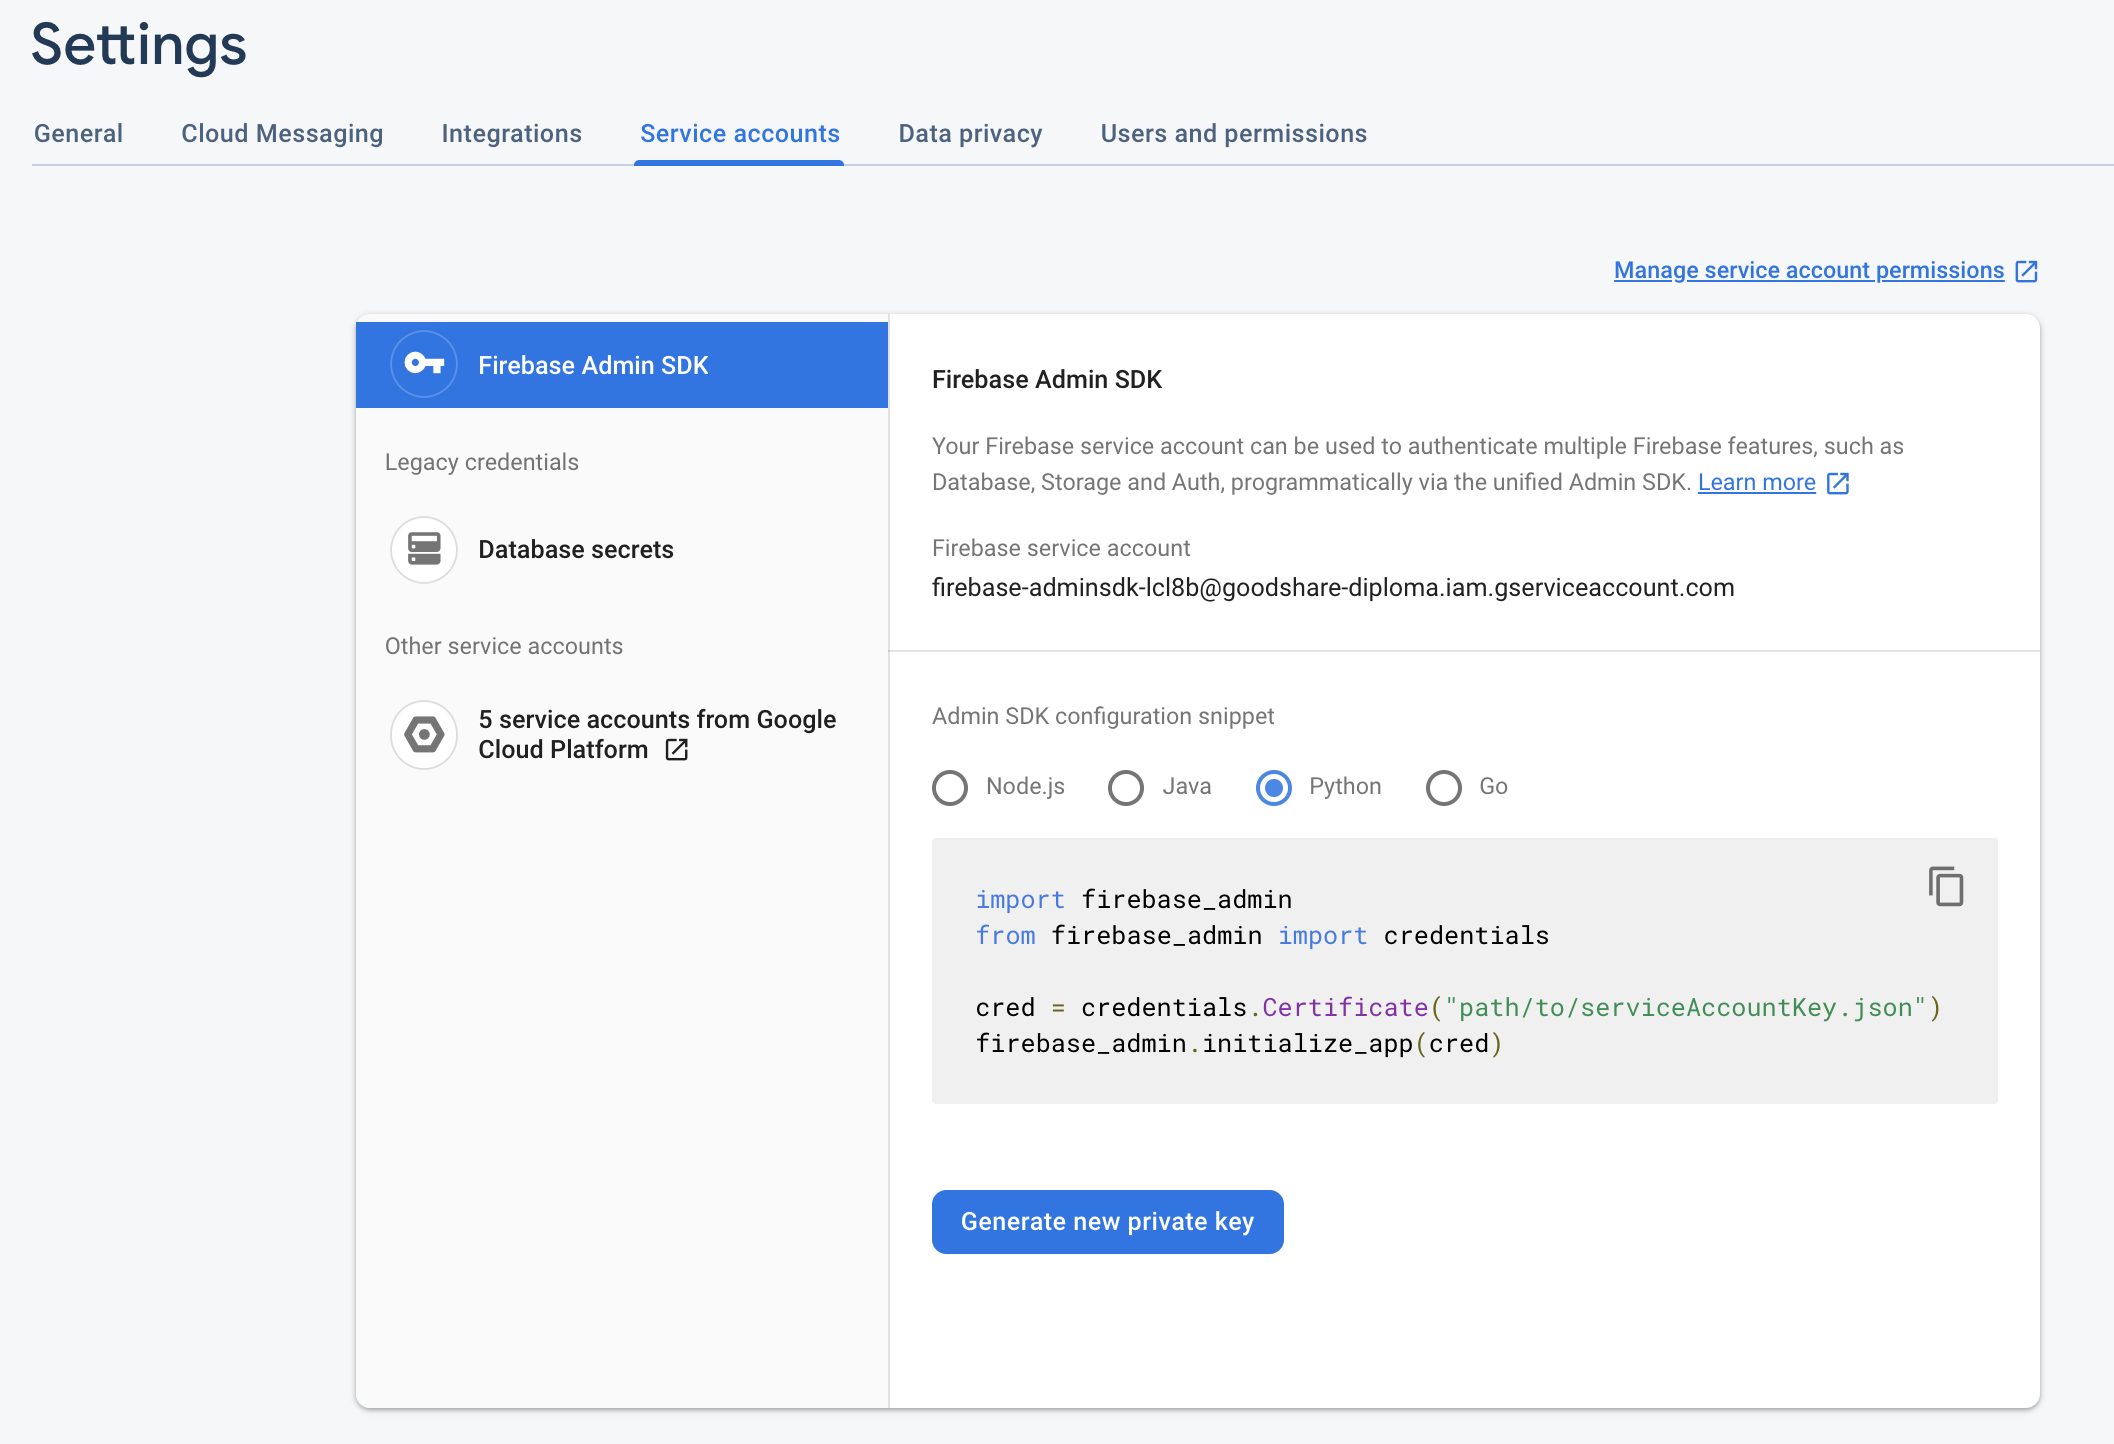
\includegraphics[scale=0.4]{service_file.png}
    \caption{ Графический интерфейс Firebase вкладки скачивания сервисного файла }
    \label{fire:admin}
\end{figure}

Далее данный файл используется для инициализации проекта (см рисунок \ref{fire:server:init}).

\begin{figure}[ht]
    \centering
    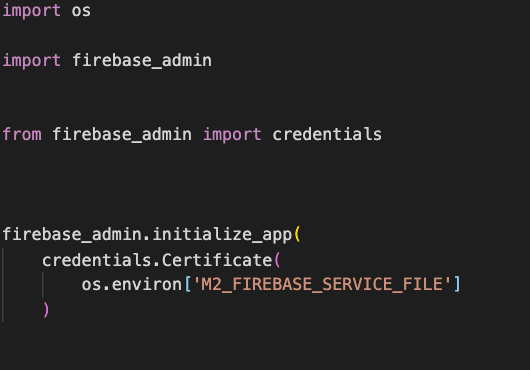
\includegraphics[scale=0.5]{init_server.png}
    \caption{ Инициализация Firebase на серверной части }
    \label{fire:server:init}
\end{figure}

После чего в разделах ниже будет добавлен и использован функционал данной библиотеки для реализации отправки уведомлений и организации аунтентификации по номеру телефона.


В целях соблюдения концепции <<Двенадцать факторов>>, а так же облегчения развертывания проекта, инициализация проекта клиентской части происходит с помощью переменных окруженя.
Как и для серверной части, данные доступа приложения можно получить в панели администратора Firebase.

Для того, чтобы облегчить процесс использования сервисов Firebase на клиентской части, был написан сервис Firebase(см рисунок \ref{fire:front:init}).

\begin{figure}[ht]
    \centering
    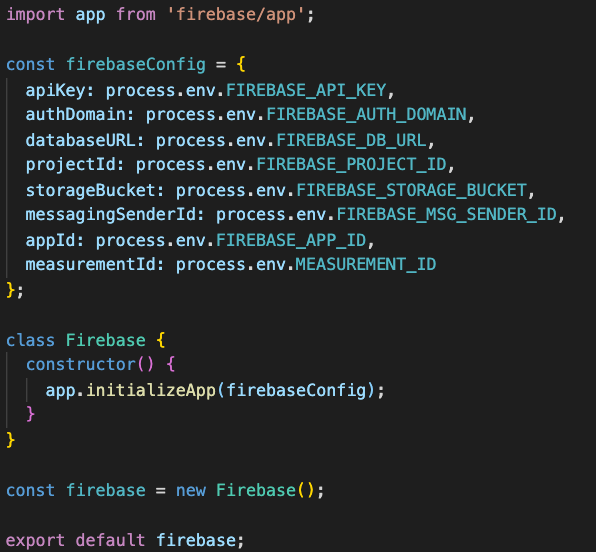
\includegraphics[scale=0.5]{firebase_front_init.png}
    \caption{ Инициализация Firebase на клиентской части }
    \label{fire:front:init}
\end{figure}

Сервис представляет собой синглтон, который предоставляет доступ к инициализированному приложению.
В разделах ниже в него будут добавлены необходимые функции.

\subsubsection{Использование Firebase Authentication}\hfill

Firebase обеспечивает службы серверной части, простые пакеты разработчика и готовые библиотеки интерфейса для аутентификации пользователей различных приложения на любых платформах.
На основе требований к ПО было принято решение использования модуля Firebase Authentication с провайдером аутентификации Phone Number.

В первую очередь был создан набор тестовых номеров телефонов, потому что при использовании одного и того же номера для аутентификации Firebase может блокировать этот номер на некоторое время.
Список созданных тестовых номеров представлен на рисунке \ref{fire:phones}.
\begin{figure}[ht]
    \centering
    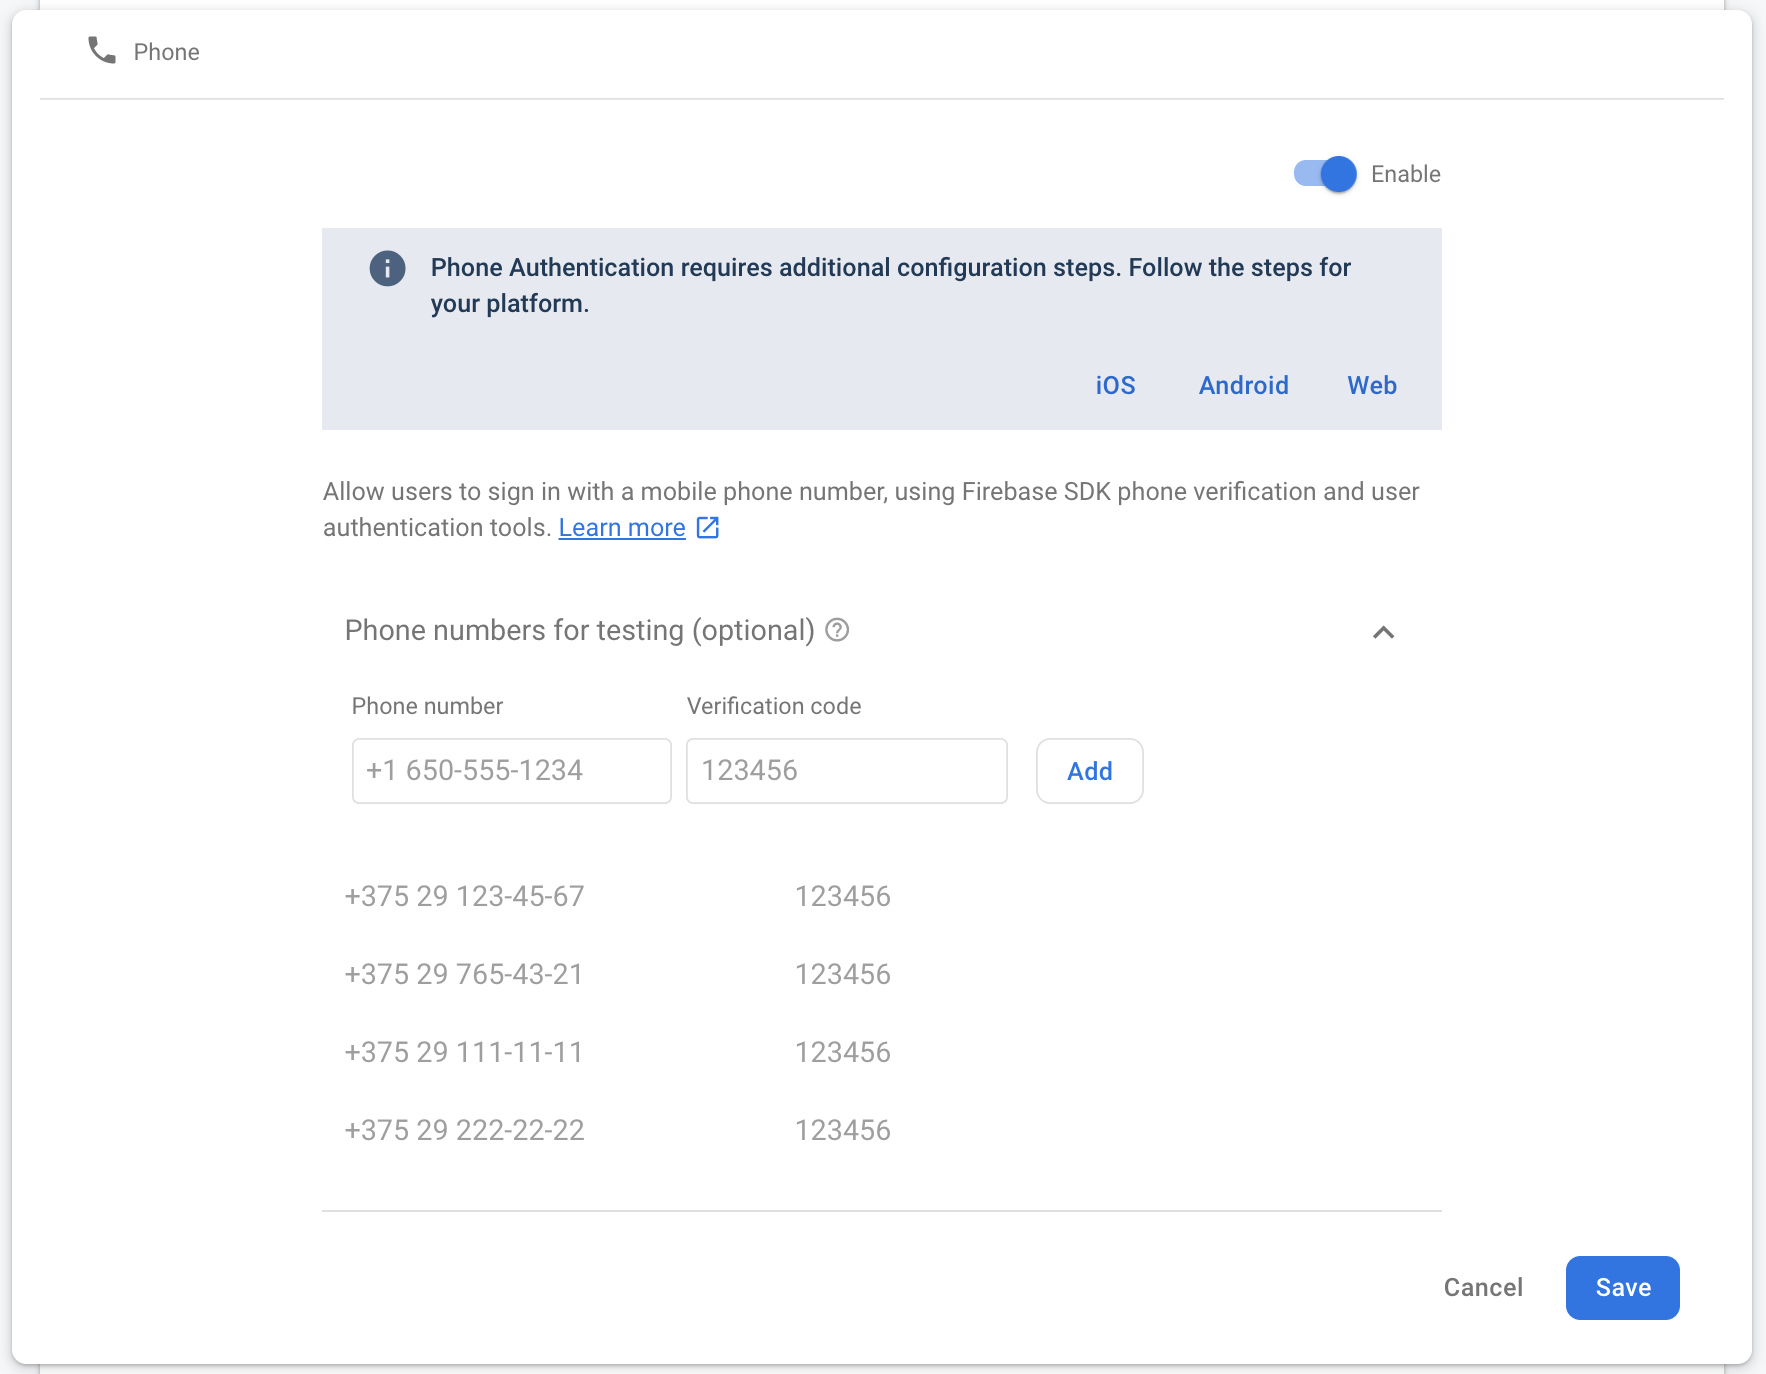
\includegraphics[scale=0.5]{firebase_phone_list.png}
    \caption{ Список используемые тестовых номеров телефонов }
    \label{fire:phones}
\end{figure}

После этого необходимо интегрировать использование аутентификации с помощью номера телефона на клиентскую часть.

Как было сказано выше, для удобного обращения к сервисам фаербейз был разработан модуль Firebase.
В нем были реализованы функции:
\begin{itemize}
    \item Выслать OTP-код на номер телефона;
    \item Проверить OTP-код;
\end{itemize}

Прежде чем войти в систему пользователей с их телефонов, необходимо настроить средство проверки рекапчи.
Firebase использует reCAPTCHA для предотвращения злоупотреблений.
Таким образов для интеграции Firebase Authentication с помощью номера телефона необходимо создать каптчу(см рисунок \ref{fire:captcha}(а)).
И так же организовать проверку с помощью клиентской библиотеки Firebase(см рисунок \ref{fire:captcha}(б)).


\begin{figure}[h]
    \centering
    \subfloat[]{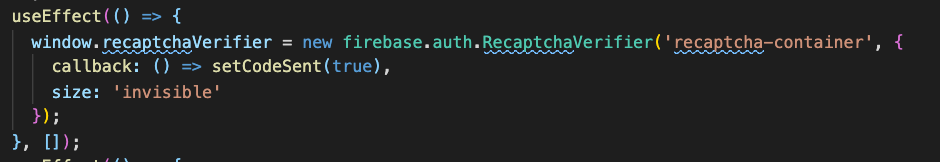
\includegraphics[scale=0.8]{firebase_recaptcha.png}} \\
    \subfloat[]{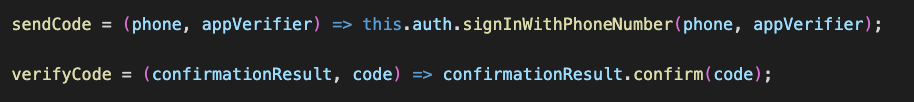
\includegraphics[scale=0.8]{firebase_auth_code.png}}
    \caption{ (a) - Интеграция reCAPTCHA в форму аунтентификации, (б) - Интеграция функционала для работы с аунтентификацией по номеру телефона }
    \label{fire:captcha}
\end{figure}


После успешной проверки OTP-кода Firebase генерирует IdToken, котрый представляет собой JWT токен.
Данный токер вместе с номером телефона отправляется на серверную часть для получения токена авторизации.

Для обработки процесса аунтентификации пользователя на серверной части была реализована проверка IdToken с помощью серверной библиотеки Firebase.


Был написан сериализатор(см рисунок \ref{server:seri}), который средствами серверной библиотеки Firebase распаковывает IdToken и проверяет, соответствие номера телефона запроса с номером телефона в токене.
\begin{figure}[h!]
    \centering
    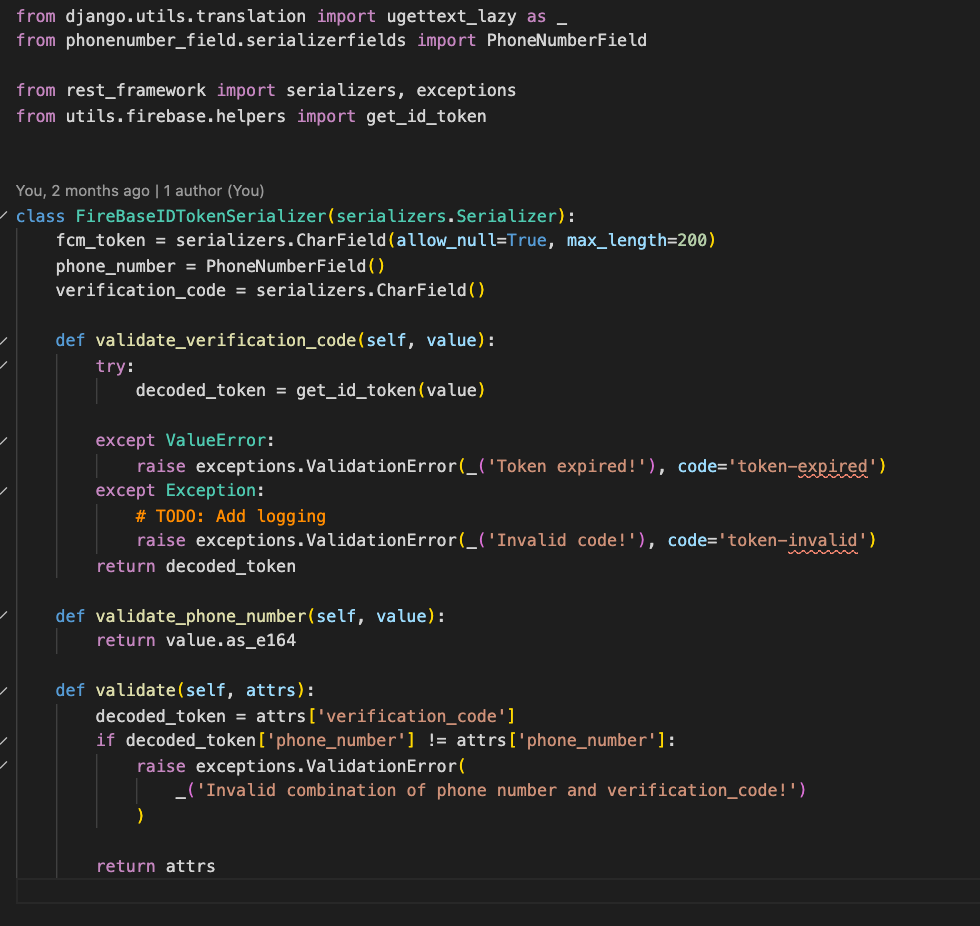
\includegraphics[clip, scale=0.8]{firebase_backend_token.png}
    \caption{ Сериализатор запроса аутентификации пользователя }
    \label{server:seri}
\end{figure}

При неуспешной обработке токена сервер возвращает 40X ответ клиентской части с описанием ошибки.
При успешной обработке токена сервер генерирует токен авторизации и возвращает его в ответе.

\subsubsection{Использование Firebase Messaging}\hfill

Firebase Cloud Messaging (FCM) - это кросс-платформенное решение для обмена сообщениями, которое позволяет  отправлять сообщения без каких-либо затрат.

На серверной части была написана утилита для отправки уведомлений как одному пользователю, так и многим (см рисунок \ref{server:sendpush}).

\begin{figure}[h]
    \centering
    \subfloat[]{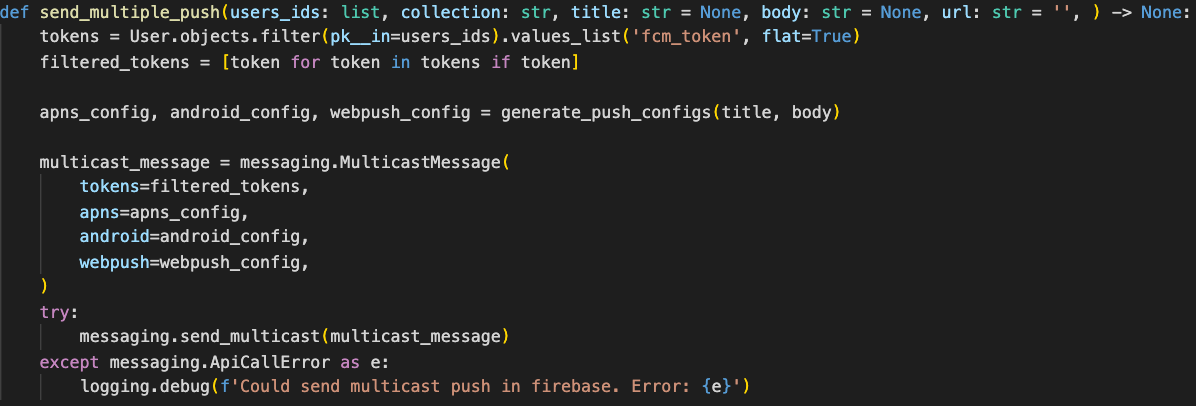
\includegraphics[scale=0.8]{server_send_multiple.png}} \\
    \subfloat[]{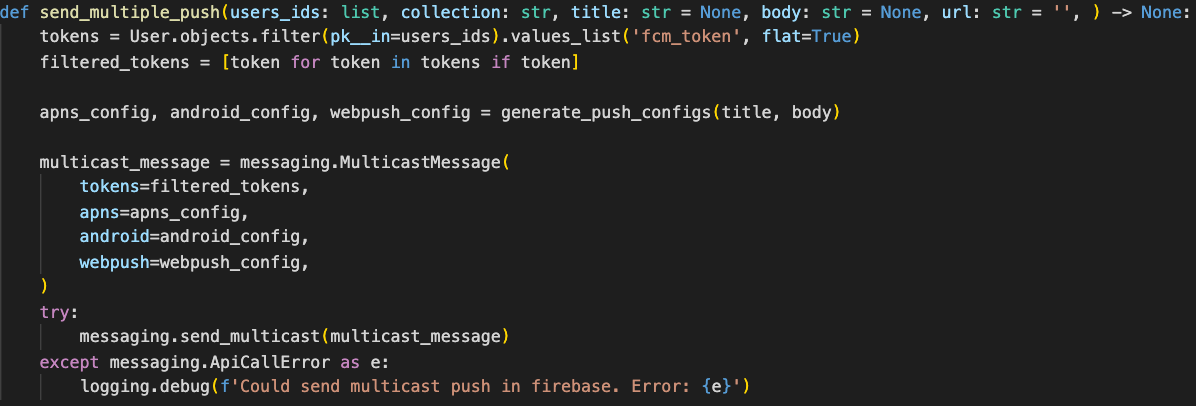
\includegraphics[scale=0.8]{server_send_multiple.png}}
    \caption{ (a) - Отправка уведомления одному пользователю, (б) - Отправка уведомления нескольким пользователям }
    \label{server:sendpush}
\end{figure}

Токен для отправки уведомлений обновляется при аутентификации пользователя в системе.
Во избежании ошибок при отправке уведомлений была добавлена проверка на наличие FCM токена у пользователя.

\subsection{Развертывание программного обеспечения}
В первую очередь стоит обратить внимание на то, что данный проект состоит из трех компонент:
\begin{itemize}
    \item Клиентское приложение;
    \item Серверное приложение;
    \item База данных.
\end{itemize}

При том изобилии компонент, которое у имеется, решением для разработки было использование docker-compose.
Таким образом был написан <<docker-compose.yml>> файл(см рисунок \ref{composefile}).

\begin{figure}[h!]
    \centering
    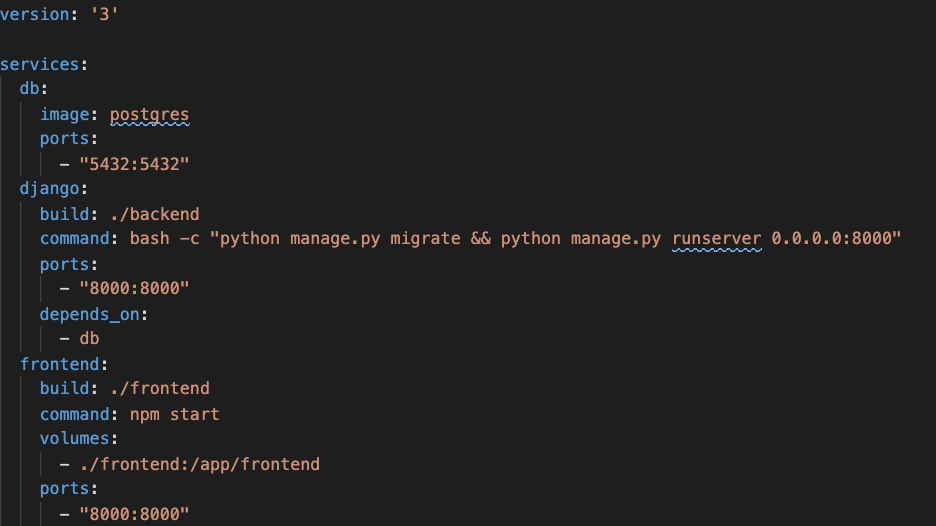
\includegraphics[clip, scale=0.8]{doc-compose.png}
    \caption{ Docker-compose файл }
    \label{composefile}
\end{figure}
docker-compose

Данный файл состоит соответственно из трех сервисов: клиентское приложние, серверное приложение и база данных.
Стоит обратить внимание, что серверное приложение не может быть запущено, пока не запущена база данных.
так же клиентское приложение не может быть запущено, пока не запущено серверное приложеие.
Во избежании увеличения размера файла было решено хранить переменные окружения в образах самих сервисов.

Далее были написаны файлы Dockerfile для клиентского и сервеного приложений(см рисунок \ref{dockerfiles}).

\begin{figure}[h]
    \centering
    \subfloat[]{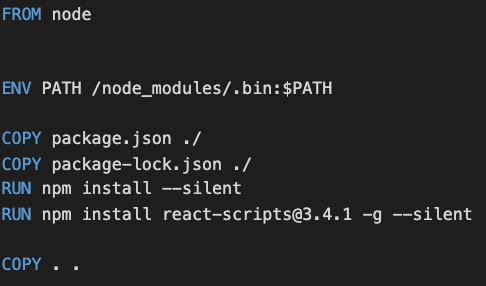
\includegraphics[scale=0.9]{doc-front.png}} \\
    \subfloat[]{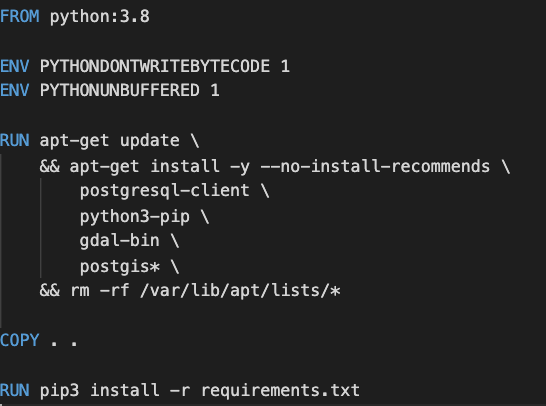
\includegraphics[scale=0.8]{doc-back.png}}
    \caption{ (a) - Dockerfile клиентского приложения, (б) - Dockerfile серверного приложения }
    \label{dockerfiles}
\end{figure}

Таким образом командой <<docker-compose up>> можно запустить проект.
